\documentclass[12pt, a4paper]{article}
\usepackage[czech]{babel}

\usepackage{graphicx}
\usepackage{parskip}
\usepackage{longtable}
\usepackage{amsmath}
\usepackage{float}
\usepackage{url}
\usepackage{microtype}
\usepackage[margin=2cm]{geometry}

\usepackage[backend=biber,style=authoryear]{biblatex}
\addbibresource{zdroje.bib}

\begin{document}

\begin{titlepage}
    \centering
    {\large UNIVERZITA KARLOVA\par}
    \vspace{0.2cm}
    {\large {Přírodovědecká fakulta}\par}
    \vspace{0.2cm}
    {\large Katedra aplikované geoinformatiky a kartografie\par}

    \vspace{2cm}

    {\large Studijní program:\par}
    \vspace{0.2cm}
    {\large Geoinformatika, kartografie a dálkový průzkum Země\par}

    \vspace{2cm}

    
\includegraphics[width=5cm]{logo.png}\par

    \vspace{1cm}

    {\large \textbf{Jakub Fuchsig, Šimon Kohout}\par}
    \vspace{1cm}
    {\Large \textbf{Úloha 2: Konstrukce polyedrických glóbů }\par}
    \vspace{2cm}  
    {\large Ústí nad Labem, Zákupy\par} 
\end{titlepage}

\section{Zadání}
Vybraná platonská tělesa (šestistěn, čtyřstěn a osmistěn nebo dvanáctistěn) použijte pro polyedrickou aproximaci sféry.

Na plošky platonských těles znázorněte v gnomonické projekci
\begin{align*}
x &= R \cdot \tan(90^{\circ} - \tilde{s})\cos d, \\
y &= R \cdot \tan(90^{\circ} - \tilde{s})\sin d
\end{align*}
geografickou síť doplněnou zákresem kontinentů. Skript pro generování sítě poledníků, rovnoběžek a znázornění kontinentů realizujte v programu MATLAB bez použití externích funkcí. Soubory se zákresem kontinentů exportujte z vhodné datové sady.

Vytvořte prostorové modely polyedrických globů v měřítku 1:100 000 000 nebo 1:50 000 000 dle možnosti Vaší tiskárny a pošlete fotografii/video Vašeho glóbu. Součástí úlohy bude příloha s rozloženými modely globů.

Zjistěte následující vlastnosti gnomonické projekce v okrajovém bodě Q jedné ze stěn Platonského tělesa:
\begin{itemize}
    \item měřítko $m_{p}$ v poledníku, měřítko $m_{r}$ v rovnoběžce,
    \item poloosy $a, b$ Tissotovy indikatrix,
    \item úhel $\omega^{\prime}$ mezi obrazem poledníku a rovnoběžky,
    \item maximální úhlové zkreslení $\Delta\omega$,
    \item měřítko ploch $P$.
\end{itemize}

Vypočtené parametry v bodě Q použijte k zákresu Tissotovy indikatrix (doporučené měřítko 1:1 000 000), jako podklad využijte obraz geografické sítě na příslušné stěně Platonského tělesa v gnomonické projekci, volte $\Delta u = \Delta v = 10^{\circ}$ (formát A4, popř. odpovídající).

Výpočty proveďte pro referenční kouli s poloměrem $R = 6380$ km, hodnoty měřítek a poloos Tissotovy indikatrix uveďte s přesností na 6 desetinných míst, úhlové hodnoty s přesností na vteřiny ("). Výsledky zkontrolujte s hodnotami získanými z programu Proj.4.
\vspace{1em}
\vspace{1em}
\vspace{1em}
\vspace{1em}
\vspace{1em}

\section{Bonusové úlohy}
\begin{small}
\begin{longtable}{|p{12cm}|c|}
    \hline
    \textbf{Krok} & \textbf{Hodnocení} \\
    \hline
    \endfirsthead
    
    \hline
    \textbf{Krok} & \textbf{Hodnocení} \\
    \hline
    \endhead

    Konstrukce polyedrických globů (4- a 8- nebo 12-stěn). & 20b \\
    \hline
    Digitální 3D model globu. & +10b \\
    \hline
    Mapa na povrchu globu. & +5b \\
    \hline
    Výpočet meridiánové konvergence. & +5b \\
    \hline
    Kontrola zkreslení v knihovně Proj.4. & +15b \\
    \hline
    \textbf{Max celkem:} & \textbf{55b} \\
    \hline
\end{longtable}
\end{small}
\newpage
\clearpage



\section{Platónská tělesa}
Platonská tělesa jsou konvexní mnohostěny v trojrozměrném prostoru, které se vyznačují maximální možnou mírou symetrie. Pro tato tělesa platí dvě základní pravidla: Všechny jejich stěny jsou tvořeny naprosto shodnými pravidelnými mnohoúhelníky (n-úhelníky) a v každém vrcholu se setkává vždy stejný počet stěn a hran. Díky této pravidelnosti lze každému platonskému tělesu opsat i vepsat kulovou plochu (sféru).

Matematicky za použití Eulerovy věty o mnohostěnech, která definuje vztah mezi počtem vrcholů $V$, hran $E$ a stěn $F$ rovnicí:
$$V - E + F = 2$$
Díky tomu lze dokázat, že takových pravidelných těles může v trojrozměrném prostoru existovat právě pět.

\begin{itemize}
    \item \textbf{Čtyřstěn} (tetraedr) -- 4 stěny tvořené rovnostrannými trojúhelníky
    \item \textbf{Šestistěn} (hexaedr neboli krychle) -- 6 stěn tvořených čtverci
    \item \textbf{Osmistěn} (oktaedr) -- 8 stěn tvořených rovnostrannými trojúhelníky
    \item \textbf{Dvanáctistěn} (dodekaedr) -- 12 stěn tvořených pravidelnými pětiúhelníky
    \item \textbf{Dvacetistěn} (ikosaedr) -- 20 stěn tvořených rovnostrannými trojúhelníky
\end{itemize}
    \begin{figure}[H]
        \centering
        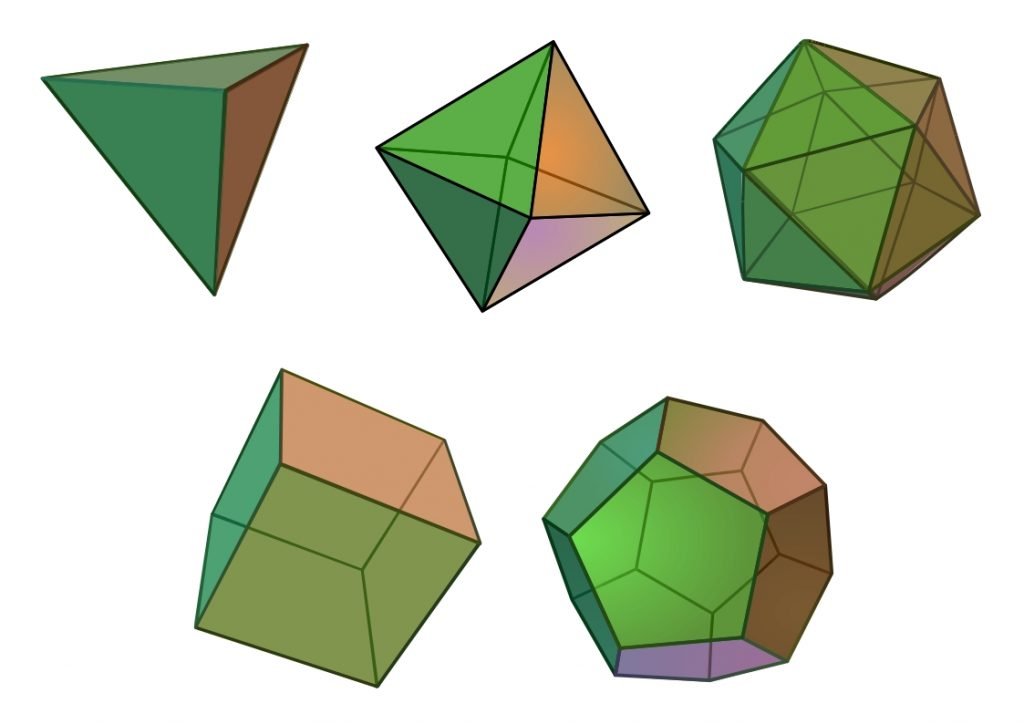
\includegraphics[width=0.75\linewidth]{Platonska_telesa.jpg}
        \caption{Platonská tělesa: čtyřstěn, osmistěn,  dvacetistěn, krychle (šestistěn), dvanáctistěn \parencite{bayer}} 
        \label{fig:placeholder}
    \end{figure}
V matematické kartografii nacházejí platónská tělesa velmi specifické uplat\-ně\-ní. Vzhledem k tomu, že jejich středem lze proložit sféru, na kterou přiléhají, používají se jako mezistupeň při tvorbě polyedrických mapových zobrazení. Sféra představující Zemi se promítne na povrch tělesa, které se následně rozvine do roviny, čímž vznikne rovinná mapa rozdělená na jednotlivé trojúhelníky či čtverce.

\subsection{\textbf{Dvanáctistěn}}
Dvanáctistěn je jedním z nejzajímavějších platónských těles, jehož povrch je tvořen 12 shodnými pravidelnými pětiúhelníky (n = 5). V kartografii představuje aproximaci sféry, ovšem za cenu složitějšího matematického postupu při výpočtu souřadnic a konstrukci sítě. Dvanáctistěn byl zvolen jako těleso pro tuto úlohu.
\begin{itemize}
    \item \textbf{Počet stěn ($F$):} 12 (pravidelné n-úhelníky pro $n=5$),
    \item \textbf{Počet hran ($E$):} 30
    \item \textbf{Počet vrcholů ($V$):} 20
\end{itemize}
\subsubsection{Geometrie stěny a vnitřní úhly}

Analýza geometrie vyžaduje určení vnitřního úhlu $\omega$ pravidelného pětiúhelníku o délce hrany $a$. Tento úhel mezi dvěma sousedními stranami určíme vztahem:
\[ \omega = \frac{(n-2)\pi}{n} = \frac{3\pi}{5} = 108^\circ \]


Pro konstrukci plošky v gnomonické projekci je zásadní znalost délky stěnové úhlopříčky $u_s$. Využitím kosinové věty v rovnoramenném trojúhelníku (tvořeném dvěma stranami a úhlopříčkou) získáme:
\[ u_s^2 = 2a^2(1 - \cos \omega) \]

Vzhledem k tomu, že $\cos 108^\circ = -\frac{1}{1+\sqrt{5}}$, lze vztah zjednodušit a vyjádřit pomocí \textbf{zlatého řezu} ($\phi \approx 1,618$):
\[ u_s = a \frac{1+\sqrt{5}}{2} = a \cdot \phi \]


\subsubsection{Úhel mezi stěnami a kartografické póly}
Důležitým parametrem pro určení polohy stěn je úhel $\alpha$ mezi dvěma sousedními ploškami dvanáctistěnu. V návodu \cite{bayer} je tento úhel odvozen pomocí konstrukce pomocného čtyřbokého jehlanu nad hranou tělesa. Pro tento úhel platí vztah:
\[ \sin\frac{\alpha}{2} = \frac{u_s}{2v} = \frac{2}{\sqrt{10-2\sqrt{5}}} \approx 56,5825^\circ \implies \alpha \approx 116,5651^\circ \]

Středy jednotlivých plošek představují tzv. kartografické póly $K$, které jsou body dotyku vepsané sféry. Zeměpisná šířka těchto pólů pro pět plošek nad rovníkem (severní polokoule) se určí jako:
\[ u_{\alpha} = \alpha - 90^\circ \approx 26,5651^\circ \]
Zbývajících pět plošek na jižní polokouli má zeměpisnou šířku symetricky sdruženou $u_j = -u_{\alpha}$ a zbylé dvě plošky se nacházejí přímo v severním a jižním pólu \cite{bayer}.



\subsubsection{Poloměry vepsané a opsané sféry}
Pro gnomonickou projekci, která se při konstrukci polyedrických glóbů používá, je určující poloměr vepsané sféry $\rho$. Ten představuje vzdálenost středu tělesa od dotykového bodu $U$ v těžišti každé stěny:
\[ \rho = \rho_s \tan\frac{\alpha}{2} = \frac{a}{20}\sqrt{10(25+11\sqrt{5})} \]

Poloměr opsané sféry $r$, která prochází všemi 20 vrcholy dvanáctistěnu, vypočteme z pravoúhlého trojúhelníku tvořeného poloměrem opsané kružnice stěny $r_s$ a poloměrem vepsané sféry $\rho$:
\[ r = \sqrt{r_s^2 + \rho^2} = \frac{\sqrt{3}(1+\sqrt{5})}{4}a \]

\subsubsection{Zeměpisné souřadnice vrcholů}
Aby bylo možné plošky správně oříznout, je nutné znát zeměpisné souřadnice všech 20 vrcholů. Podle \cite{bayer} jsou vrcholy rozděleny do čtyř výškových úrovní (přičemž v každé úrovni je 5 vrcholů s odlehlostí $72^\circ$):
\begin{enumerate}
    \item \textbf{Vrcholy $P$ až $T$:} horní prstenec se zeměpisnou šířkou $u_{\gamma} = 90^\circ - \gamma \approx 52,6226^\circ$
    \item \textbf{Vrcholy $G, I, K, M, O$:} střední severní prstenec se šířkou $u_{\delta} \approx 10,8123^\circ$
    \item \textbf{Vrcholy $F, H, J, L, N$:} střední jižní prstenec se šířkou $u_j = -u_{\delta}$
    \item \textbf{Vrcholy $A$ až $E$:} dolní prstenec se šířkou $u_j = -u_{\gamma}$
\end{enumerate}

\begin{figure}[H]
    \centering
    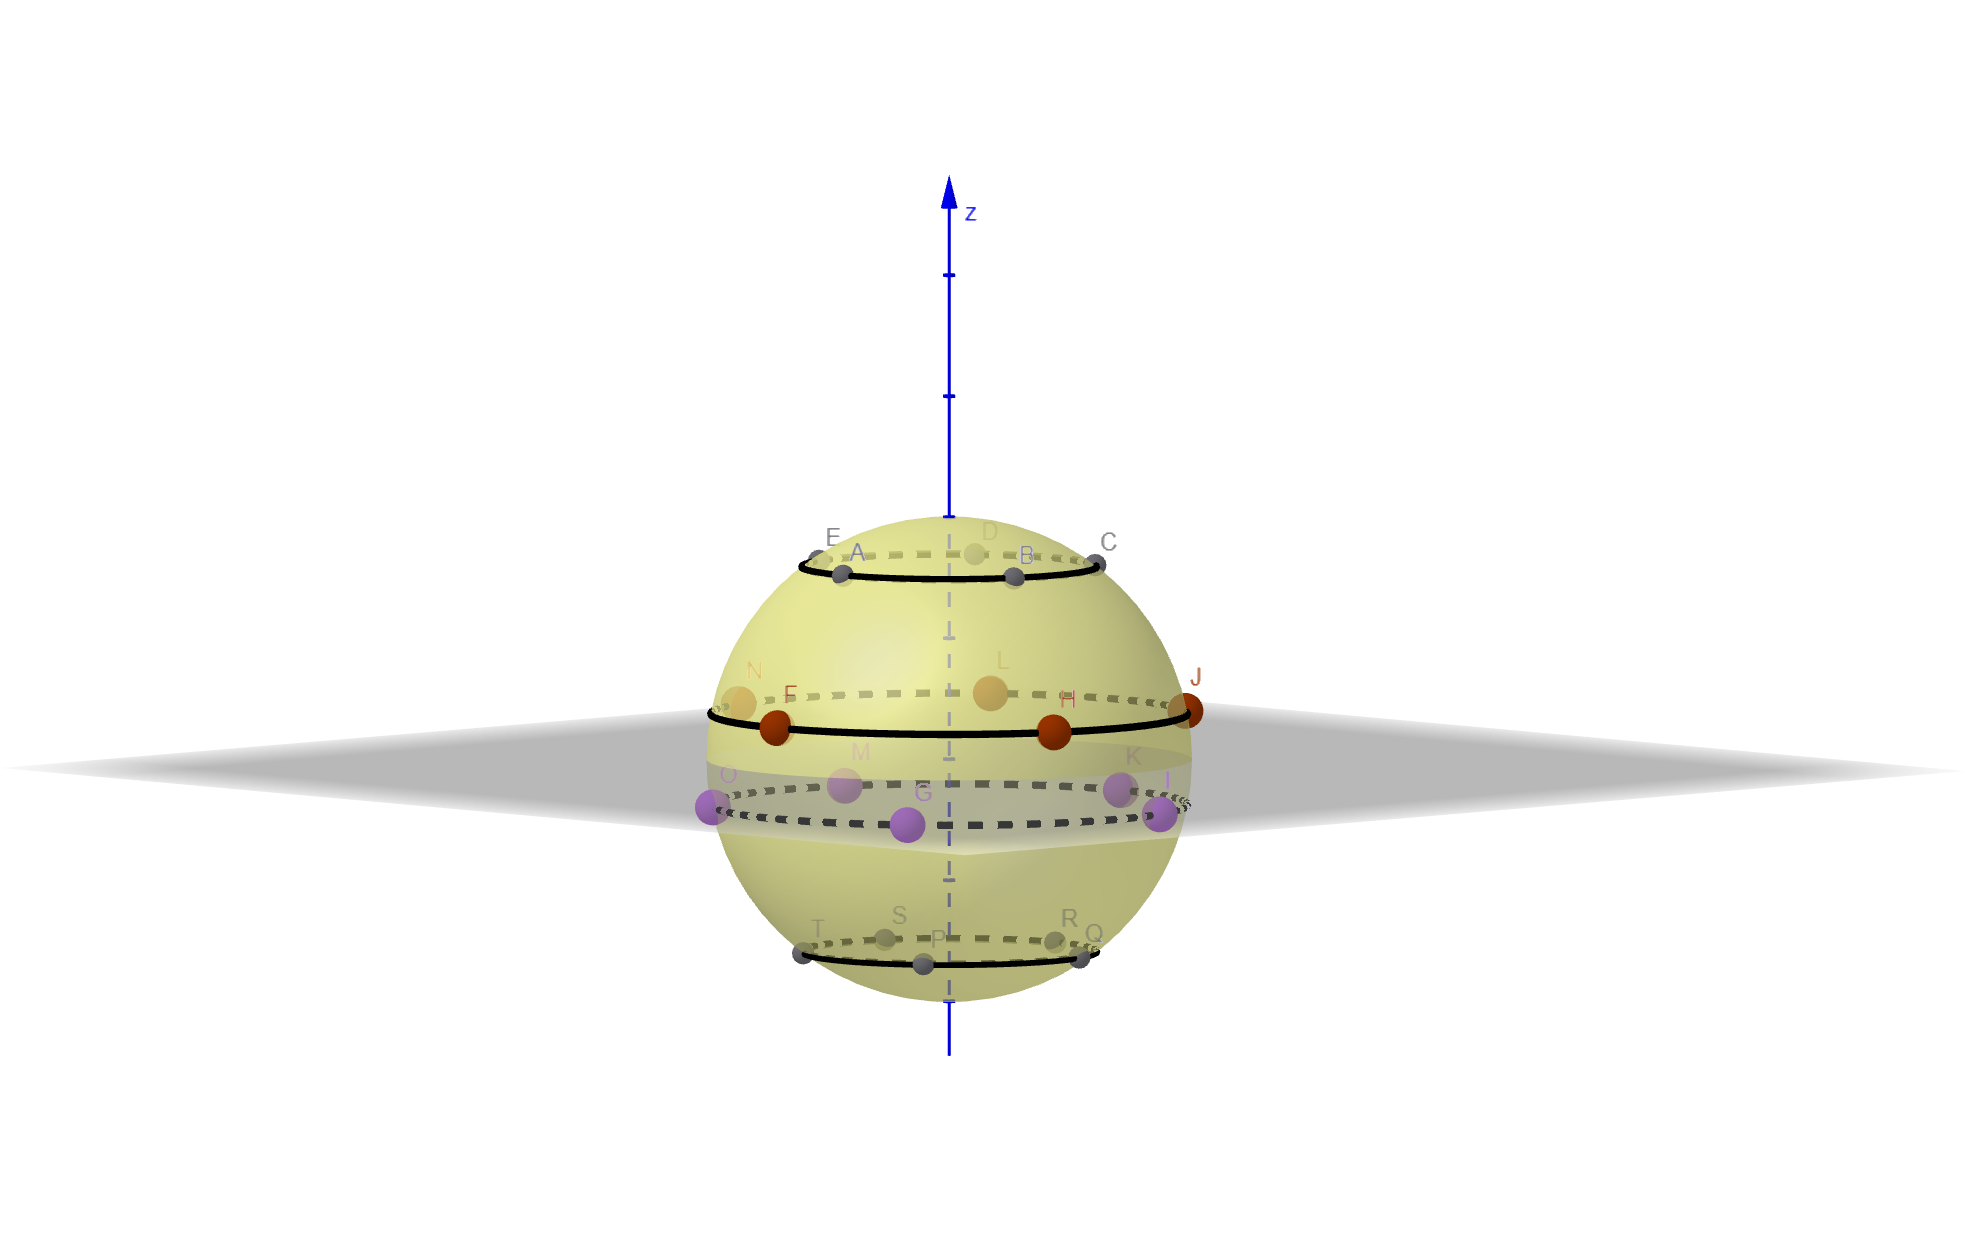
\includegraphics[width=1\linewidth]{geogebra-export.png}
    \caption{Vizualizace čtyř prstenců zeměpisných šířek vrcholů dvanáctistěnu na sféře}
    \label{fig:geogebra_vertices}
\end{figure}
\newpage
\clearpage

\begin{table}[H]
\centering
\caption{Zeměpisné souřadnice vrcholů dvanáctistěnu (orientace dle GeoGebry)}
\label{tab:souradnice_oprava}
\begin{tabular}{|c|c|r|r|}
\hline
\textbf{Prstenec} & \textbf{Vrchol} & \textbf{Zeměp. šířka $u$} & \textbf{Zeměp. délka $v$} \\ \hline
& $A$ & $52,6226^\circ$ & $0^\circ$ \\
& $B$ & $52,6226^\circ$ & $72^\circ$ \\
\textbf{Horní } & $C$ & $52,6226^\circ$ & $144^\circ$ \\
 & $D$ & $52,6226^\circ$ & $216^\circ$ \\
& $E$ & $52,6226^\circ$ & $288^\circ$ \\ \hline
& $F$ & $10,8123^\circ$ & $0^\circ$ \\
& $H$ & $10,8123^\circ$ & $72^\circ$ \\
\textbf{Střední severní} & $J$ & $10,8123^\circ$ & $144^\circ$ \\
& $L$ & $10,8123^\circ$ & $216^\circ$ \\
& $N$ & $10,8123^\circ$ & $288^\circ$ \\ \hline
& $G$ & $-10,8123^\circ$ & $36^\circ$ \\
& $I$ & $-10,8123^\circ$ & $108^\circ$ \\
\textbf{Střední jižní} & $K$ & $-10,8123^\circ$ & $180^\circ$ \\
& $M$ & $-10,8123^\circ$ & $252^\circ$ \\
& $O$ & $-10,8123^\circ$ & $324^\circ$ \\ \hline
& $P$ & $-52,6226^\circ$ & $36^\circ$ \\
& $Q$ & $-52,6226^\circ$ & $108^\circ$ \\
\textbf{Dolní} & $R$ & $-52,6226^\circ$ & $180^\circ$ \\
 & $S$ & $-52,6226^\circ$ & $252^\circ$ \\
& $T$ & $-52,6226^\circ$ & $324^\circ$ \\ \hline
\end{tabular}
\end{table}

\section{Gnómonická projekce}
Jedná se o jednoduché azimutální zobrazení, ve kterém se každý bod ležící na sféře promítá ze středu sféry na rovinu, která se na sféru tečná v kartografickém pólu. Tento pól v normální poloze odpovídá severnímu pólu. Na obrázku \textbf{XYZ} lze pozorovat princip daného zobrazení. Obraz bodu $P$ ležící na sféře s poloměrem $\rho$ se zobrazuje na rovinu jako bod $P'$. 

\begin{figure}[H]
        \centering
        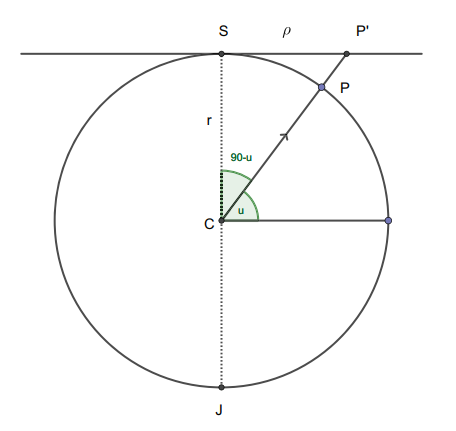
\includegraphics[width=0.5\linewidth]{gnom.png}
        \caption{Gnómonická projekce v normální poloze \parencite{bayer}} 
        \label{fig:placeholder}
        
    \end{figure}

Pro toto zobrazení platí tedy zobrazovací rovnice:
$$
\rho = rtan(90^{\circ}-u), \quad\epsilon = v
$$
kde $r$ je poloměr sféry a $u,v$ jsou původní souřadnice bodu.

Pokud se vezme obecná poloha zobrazení, pak se zobrazovací rovnice změní na tento tvar:
$$
\rho = rtan((90^{\circ}-\text{š}), \quad\epsilon = d
$$
kde $\text{š},d$ jsou kartografické souřadnice bodu.

Při převodu zobrazení do pravoúhlého tvaru vznikne takováto rovnice:
$$
x = Rtan(90^{\circ}-\text{š})cos(d), \quad y = Rtan(90^{\circ}-\text{š})sin(d)
$$

Díky svým vlastnostem se v tomto zobrazení poledníky zobrazí jako polopřímky vycházející z pólu a rovnoběžky se zobrazí jako soustředné kružnice k pólu. Gnómonické zobrazení má jednu nevýhodu a to, že lze zobrazit pouze jednou polokouli a nelze zobrazit rovník, jelikož platí:

$$\lim_{u \to \pm 0} \tan(90^\circ - u) = \pm\infty.$$

\subsection{Vlastnosti projekce}
Každé zobrazení a projekce má své specifické vlaasatnosti, díky kterým se odlišuje od ostaních zobrazení. Níže jsou vypsány a popsány hlavní parametr zobrazení.

Pro teoretický podklad jednotlivých vlastností je důležité spočítat parciální derivace zobrazovacích rovnic podle proměnných $u$ a $v$. Tyto rovnice jsou $f$ a $g$, poté platí:

$$f_u = \frac{\partial f}{\partial u} = \frac{R}{\cos^2(\frac{\pi}{2} - u)}  (-1)  \cos(v)$$
$$g_u = \frac{\partial g}{\partial u} = \frac{R}{\cos^2(\frac{\pi}{2} - u)}  (-1)  \sin(v)$$
$$f_v = \frac{\partial f}{\partial v} = -R\tan\left(\frac{\pi}{2} - u\right)  \sin(v)$$
$$g_v = \frac{\partial g}{\partial v} = R\tan\left(\frac{\pi}{2} - u\right)  \cos(v)$$

\subsubsection{Měřítko $m_p$ v poledníku}
Určuje lokální měřítko ve směru poledníku, tedy deformaci mapy v tomto směru. Je dáno vztahem:

$$m_{p}^{2} = \frac{f_{u}^{2} + g_{u}^{2}}{R^{2}},$$

kam po dosazení parciálních derivací lze získat upravený vztah pro výpočet $m_p$ v gnómonické projekci:

$$m_p = \frac{1}{sin^2(u)}.$$
\subsubsection{Měřítko $m_r$ v rovnoběžce}
Obdobně určuje měřítko ve směru rovnoběžky, tedy deformaci mapy v daném sněru. Určuje se ze vztahu: 

$$m_{r}^{2} = \frac{f_{v}^{2} + g_{v}^{2}}{R^{2}cos^2(u)}$$

a opět po dosazení parciálních derivací lze získat upravený vztah pro výpočet $m_r$ pro gnómonickou projekci:

$$m_r = \frac{1}{sin^(u)}.$$

\subsubsection{Tissotova indikatrix}
Jedná se o grafické vyjádření lokálního zkreslení v určitém bodě. Určuje, jak se kružnice z referenční sféry transformuje do podoby elipsy na zobrazovací rovině. Důležitý je výpočet polos $a$ a $b$. Pro jednoduchá zobrazení však platí rovnost poloos s výše zmíněnými měřítky, tedy:

$$a = m_p, \quad b = m_r.$$

\subsubsection{Úhel $\omega'$ mezi obrazem poledníku a rovnoběžky}
Určuje úhel, pod kterým se na mapě protíná obraz poledníku s obrazem rovnoběžky. Lze vyjádřit pomocí vzorce:

$$\tan \omega' = \frac{g_u  f_v - f_u  g_v}{f_u  f_v + g_u  g_v}.$$

Po dosazení parciálních derivací ve jmenovateli vyjde nula, jedná se tedy o \textbf{ortogonální} (pravoúhlé) zobrazení a platí:

$$tan(\omega') = \pm \infty \quad \to \quad \omega' = \pm \frac{\pi}{2} = 90°$$

\subsubsection{Maximální úhlové zkreslení $\Delta\omega$}
Úhlové zkreslení udává rozdíl mezi skutečným úhlem a daným úhlem na mapě. Maximální úhlové zkreslení pak udává největší možný rozdíl mezi těmito úhly v daném bodě. Lze vypočítat podle vztahu:

$$sin\frac{\Delta\omega}{2}=\frac{|b-a|}{b+a}=\frac{|m_{r}-m_{p}|}{m_{r}+m_{p}}.$$

Po dosazení získáme vztah:

$$\Delta\omega=\frac{sin(u-1)}{sin(u+1)}.$$

\subsubsection{Měřítko ploch $P$}
Měřítko ploch $P$ udává poměr diferenciální plošky na mapě a na referenční sféře, tedy kolikrát se plocha na mapě zmenší/zvětší. Lze vypočítat jako:

$$P = \frac{g_u f_v - f_u g_v}{R^2 \cos u}$$

Jelikož gnómonická projekce patří do jednoduchých zobrazení, platí: 

$$P = m_p m_r$$

a po dosazení lze získat přímo měřítko ploch pro naši projekci:

$$P = \frac{1}{\sin^3 u}$$

\subsubsection{Meridiánová konvergence $c$}
Jendá se o rozdíl mezi mezi směrem základního a místního poledníku v daném bodě, tedy jak moc se liší obraz místního poledníku v obraze od svislé osy $y$. Pro výpočet je nutné vypočítat směrnici poledníku $\sigma_p$:

$$\tan \sigma_p = \frac{g_u}{f_u},$$

po dosazení a upravě platí: 

$$\sigma_p = v$$

Po vyčíslení lze získat meridiánová konvergence jako:

$$c = | \sigma_p - \frac{\pi}{2} = |\sigma_p - \frac{\pi}{2}|,$$

kde $\sigma_0$ je směrnice základního poledníku $\sigma_0 = \frac{\pi}{2}$.

\clearpage
\newpage
\section{Konstrukce polyedrických glóbů}

Konstrukce polyedrického globu na dvanáctistěnu představuje proces, při kterém je sféra (Země) rozdělena na 12 částí, z nichž každá je samostatně zobrazena do roviny příslušné plošky tělesa. Celý postup lze rozdělit do několika logických kroků, od definice parametrů až po finální sestavení modelu.

\subsection{Definice měřítka a poloměru sféry}
Každý model je definován měřítkovým číslem $M$, které určuje výslednou velikost globu. Poloměr sféry vepsané dvanáctistěnu $r$, který následně vstupuje do zobrazovacích rovnic, se určí jako:
\[ r = \frac{R}{M}, \]
kde $R$ je poloměr náhradní sféry pro aproximaci Země (standardně se používá hodnota $R = 6\,378\,000$ m). Hodnota $r$ pak odpovídá skutečné vzdálenosti od středu modelu k těžišti každé plošky, kde je zkreslení zobrazení nulové.

\subsection{Význam zobrazení}
Výběr gnómonické projekce pro tvorbu polyedrických modelů je podmíněn její unikátní geometrickou vlastností, která přímo umožňuje fyzickou globu. Jelikož hrany dvanáctistěnu leží na hlavních kružnicích sféry (ortodromách), jejich obrazem v rovině každé plošky jsou opět úsečky. Každá ploška dvanáctistěnu má svůj vlastní kartografický pól $K$, který je umístěn do jejího těžiště. Díky tomuto postupu lze vytvořit spojitý povrch globu, kde kresba polohopisu i geografické sítě plynule přechází přes hrany tělesa bez nutnosti grafických korekcí. Gnomonická projekce je však schopna zobrazit vždy pouze část sféry, což pro potřeby dvanáctistěnu, kde každá ploška zabírá jen malou část povrchu, plně vyhovuje.

\subsection{Tvorba geografické sítě}
Na každé plošce se geografická síť vytváří v obdélníkové oblasti definované intervaly $\langle \min u, \max u \rangle \times \langle \min v, \max v \rangle$. Při generování sítě je nutné stanovit parametry určující vzdálenosti mezi poledníky a rovnoběžkami ($\Delta u, \Delta v$) a jemnost vzorkování jednotlivých čar ($\delta u, \delta v$). Pro účely této práce byly použity standardní hodnoty doporučené v návodu:

\[\Delta u = \Delta v = 10^\circ, \quad \delta u = \delta v = 1^\circ\]

které byly aplikovány na všech 12 plošek dvanáctistěnu.

Rozsah oblasti $(\min, \max)$ je určen podle souřadnic vrcholů příslušné plošky. Aby poledníky a rovnoběžky pokrývaly celou plochu pětiúhelníku i po transformaci, dolní meze se volí o několik stupňů menší a horní meze o několik stupňů vyšší než jsou krajní body plošky. Použitý posun (buffer) vůči těmto hranicím se v této práci pohybuje obvykle mezi $5^\circ$ a $10^\circ$.

\subsection{Lomové body kontinentů}
Pro vyobrazení kontinentů na mapě bylo nutné, aby jedntolivé kontinenty byly uloženy zvlášť v textových souborech (viz přiložené soubory). Tyto soubory obsahují pouze souřadnice jednotlivých bodů ($u,v$) k načtení do MATLAB.

Při načítání dat byly odebrány body, které se nacházejí blízko kartografickému rovníku. Jelikož gnómonická projekce nedokáže zobrazit rovník, tyto problémové body byly výrazně deformovány či nezobrazeny vůbec.

\section{Transformace souřadnic a generování pláště}

Aby bylo možné geografická data (poledníky, rovnoběžky a obrysy kontinentů) korektně zobrazit na jednotlivé plošky dvanáctistěnu, je nutné provést transformaci ze zeměpisných souřadnic $[\phi, \lambda]$ do obecné polohy zobrazení $[\check{s}, d]$ vztažené ke kartografickému pólu $K = [u_k, v_k]$ dané stěny.

\subsection{Transformace do obecné polohy}
Při transformaci využíváme sférickou trigonometrii v trojúhelníku tvořeném pólem sféry, kartografickým pólem a zobrazovaným bodem. Pro výpočet kartografické šířky $\check{s}$ využíváme sférickou kosinovou větu:
\[ \sin \check{s} = \sin u \sin u_k + \cos u \cos u_k \cos(v_k - v) \]

Výpočet kartografické délky $d$ je složitější, protože standardní vzorce často selhávají v určení správného kvadrantu. Pro programové zpracování (např. v Pythonu nebo Matlabu) se využívá funkce \texttt{atan2}, která zajišťuje kvadrantově korektní výsledek:
\[\tan d = \frac{\sin(v_k - v) \cos u}{\cos u \sin u_k \cos(v_k - v) - \sin u \cos u_k}\]
Syntax funkce v matlabu:
\[ d = \text{atan2}\left(\sin(v_k - v) \cos u, \cos u \sin u_k \cos(v_k - v) - \sin u \cos u_k\right) \]


\subsection{Ořezové linie a geometrie plošek}
Využíváme klíčovou vlastnost gnómonické projekce, která zobrazuje ortodromy (hlavní kružnice) jako úsečky  
\begin{itemize}
    \item Pro každou plošku jsou vypočteny rovinné souřadnice $[x, y]$ jejích pěti vrcholů 
    \item Spojením těchto bodů vzniká pětiúhelníková ořezová hranice
    \item Data vně této hranice jsou odstraněna, což zajišťuje přesné lícování sousedních plošek bez spár či překrytů 
\end{itemize}

\subsection{Filtrace polohopisu}
Vzhledem k nelinearitě zobrazení, kde pro body blížící se obzoru platí $\rho \to \infty$, je nutná filtrace dat.
\begin{itemize}
    \item Body s kartografickou šířkou $\check{s} < 5^\circ$ jsou automaticky odstraňovány 
    \item Tato filtrace předchází vzniku grafických artefaktů a chyb při vykreslování kontur kontinentů 
\end{itemize}

\subsection{Sestavení modelu}
Po vygenerování obsahu jsou jednotlivé plošky exportovány ve vektorovém formátu (PDF/EPS). V grafickém editoru jsou plošky sesazeny do výsledného pláště, vytištěny a následně slepeny do prostorového modelu. 

\clearpage
\newpage

\section{Praktická realizace v prostředí MATLAB}

\subsection{Struktura skriptů pro polyedrický glóbus}


\begin{enumerate}
    \item \textbf{Hlavní řídící skript a definice parametrů (\texttt{u2.m})}\\[0.2cm] 
   Proces konstrukce dvanáctistěnu je spouštěn hlavním skriptem \texttt{u2.m}. Zde jsou definovány veškeré klíčové parametry modelu, včetně poloměru referenční sféry ($R = 1$), kroků geografické sítě a především souřadnic kartografických pólů a hraničních vrcholů pro všech 12 plošek dvanáctistěnu. Úhlové hodnoty jsou zde pro výpočetní potřeby převáděny ze stupňů na radiány. Pro vytvoření šestistěnu (krychle) slouží alternativní řídící skript \texttt{u2\_hexahedron.m}, který funguje na totožném principu, ale jeho parametry a hranice jsou přizpůsobeny pro 6 plošek.

    \item \textbf{Transformace vzhledem ke kartografickému pólu (\texttt{uvToSd.m})}\\[0.2cm]
    Převod bodů ze standardních zeměpisných souřadnic $(u, v)$ do soustavy spjaté s kartografickým pólem konkrétní stěny $(s, d)$ zajišťuje funkce \texttt{uvTosd.m}. Výpočet využívá sférickou trigonometrii, přičemž pro spolehlivé určení správného kvadrantu u kartografické délky je implementována funkce \texttt{atan2()}.

    \item \textbf{Aplikace gnómonické projekce (\texttt{gnom.m})}\\[0.2cm]
    Vlastní promítnutí transformovaných bodů na rovinu obstarává skript \texttt{gnom.m}. Ten obsahuje základní rovnice pro gnómonickou projekci v obecné poloze:
    $$ x = R \tan\left(\frac{\pi}{2} - s\right) \cos d, \quad y = R \tan\left(\frac{\pi}{2} - s\right) \sin d $$
    Tato funkce je univerzálně volána pro všechny body sítě i kontinentů.

    \item \textbf{Vykreslování plošek (\texttt{createGlobeFace.m})}\\[0.2cm]
    Tento obsáhlý skript funguje jako manažer pro každou jednotlivou stěnu dvanáctistěnu. Volá podružné funkce pro síť a polohopis a obsahuje speciální logiku pro vizuální maskování (pomocí funkce \texttt{polyshape}), která efektivně překryje veškeré přesahy grafiky vně požadovaného pětiúhelníku bílou barvou.

    \item \textbf{Zobrazení kontinetů (\texttt{drawContinent.m})}\\[0.2cm]
    Zobrazení obrysů pevnin má na starosti skript \texttt{drawContinent.m}, který načítá textové soubory s lomovými body. Kód obsahuje důležitou filtrační podmínku, která ze zpracování vyřazuje body s kartografickou šířkou $s < 0,3$ rad (zhruba 17°). Tím se eliminuje vykreslování bodů blízko horizontu zobrazení, u kterých by gnómonická projekce vracela extrémní souřadnice.

    \item \textbf{Vykreslení ořezových linií (\texttt{boundary.m})}\\[0.2cm]
    Pro přesné ohraničení plošky slouží funkce \texttt{boundary.m}. Ta transformuje a promítne zadanou pětici vrcholů, čímž vznikne obvodový polygon sloužící jako vodicí čára pro fyzické vystřižení modelu.
\end{enumerate}

\clearpage
\newpage


\subsection{Generování geografické sítě }

Geografická síť (poledníky a rovnoběžky) je primárně počítána uvnitř funkce \texttt{graticule.m}. Síť je definována v obdélníkové pracovní oblasti $(u_{min}, u_{max}) \times (v_{min}, v_{max})$, jejíž limity jsou pro každou plošku individuálně nastaveny v nadřazeném skriptu tak, aby bezpečně pokryly tvar daného pětiúhelníku. Hustota sítě je určena rozestupy $\Delta u = \Delta v = 10^\circ$, zatímco hladký tvar křivek po projekci je zajištěn jemným krokem vzorkování $\delta u = \delta v = 1^\circ$. Každý bod čáry je iterativně transformován do lokálního kartografického systému a promítnut na rovinu.

\subsection{Obrysy kontinentů}

Zpracování kontinentů bylo navrženo napříč vícero soubory. Hlavní skript \texttt{u2.m} uchovává seznam všech textových souborů (\texttt{afr.txt}, \texttt{amer.txt} atd.) v proměnné \texttt{conts}. Funkce \texttt{createGlobeFace.m} následně pomocí cyklu (\texttt{for}) tyto soubory jeden po druhém předává funkci \texttt{drawContinent.m}. Aby byl výsledný glóbus vizuálně přehlednější, jsou polygony kontinentů po projekci vyplněny poloprůhlednou barvou pomocí standardního příkazu \texttt{fill()}.

\subsection{Výpočet vlastností gnómonické projekce v bodě Q}
Výše zmíněné vlastnosti (měřítka, zkreslení, poloosy atd.) jsou počítány ve skriptu \texttt{gnom\textunderscore distortions\textunderscore nazev\textunderscore telesa.m}. Byly tedy vytvořeny dva podobné skripty pro obě platónská tělesa. 

Pro \textbf{krychli} byl zvolen bod [35.2644°, 45°], tedy vrchol stěny krychle se severním pólem [90°]. Pro \textbf{dvanáctistěn} byl zvolen bod [52.6226°, 0°], tedy opět vrchol severní stěny tělesa.

Pro oba skripty byla další část stejná.

Pro podklad zobrazené stěny tělesa byla využita část skriptu \texttt{graticule.m} v vygenerovnání geografické sítě. Jelikož však MATLAB neobsahuje funkci k vykreslení elipsy, bylo vytvoření Tissotovy indikatrix o něco náročnější. Základem byla parametrická rovnice elipsy:

$$x' = m_p \cdot \cos(t), \quad y' = m_r \cdot \sin(t),$$

kde velikosti hlavních poloos odpovídají měřítkům v poledníku $m_p$ a v rovnoběžce $m_r$ a parametr $t \in \langle0, 2\pi\rangle$, který iteruje přes celých 360° - ve skriptu pomocí \texttt{linspace(0, 2*pi)}.

Takto prozatimní elipsu bylo nutné rotovat, aby poloosa $a$ byla orientována o úhel $\alpha$ ve směru místního poledníku bodu Q. Tento úhel byl počítán z mapových souřadnic pomocí arkus tangens - \texttt{alpha = atan2(Yq\textunderscore map, Xq\textunderscore map)}.

Pro provedení rotace byla použita matice rotace $R_E$: 

$$R_E = \begin{pmatrix} \cos\alpha & -\sin\alpha \\ \sin\alpha & \cos\alpha \end{pmatrix},$$

kde po roznásobení vzniknou rovnice:

$$x_{rot} = m_p \cos(t) \cos(\alpha) - m_r \sin(t) \sin(\alpha)$$
$$y_{rot} = m_p \cos(t) \sin(\alpha) + m_r \sin(t) \cos(\alpha)$$

Dále bylo nutné orientovanou matici posunout do daného bodu Q $[X_{q\_map}, Y_{q\_map}]$ a zvětšit ji pomocí \texttt{scale\_e}, který zajišťuje aby byla daná elipsa v zobrazení vůbec vidět. Finální rovnice pro jednotlivé body elipsy mají tvar:

$$x_e = X_{q\_map} + s \left(m_p \cos(t) \cos(\alpha) - m_r \sin(t) \sin(\alpha)\right)$$$$y_e = Y_{q\_map} + s \cdot \left(m_p \cos(t) \sin(\alpha) + m_r \sin(t) \cos(\alpha)\right)$$

Díky tomuto způsobu je možné vygenerovat Tissotovu indikatrix v libovolném bodě a podle tvaru vizuálně posoudit její parametry a zkreslení.

\clearpage
\newpage

\section{Tvorba 3D digitálního modelu}
Pro splnění bonusové části úlohy, tedy vytvoření 3D digitálního modelu glóbu, bylo nutné vhodně upravit stávající 2D skripty. Hlavním cílem bylo zachovat již otestovaný matematický aparát pro gnomonickou projekci a doplnit logiku pro prostorové skládání jednotlivých stěn Platónského tělesa (dvanáctistěnu). Pro zobrazení finálního interaktivního modelu v prohlížeči (např. na 3DViewer.net) je nutné přetáhnout do okna oba vygenerované soubory současně: \texttt{dodecahedron.obj} a \texttt{dodecahedron.mtl}.


\begin{figure}[h]
    \centering
    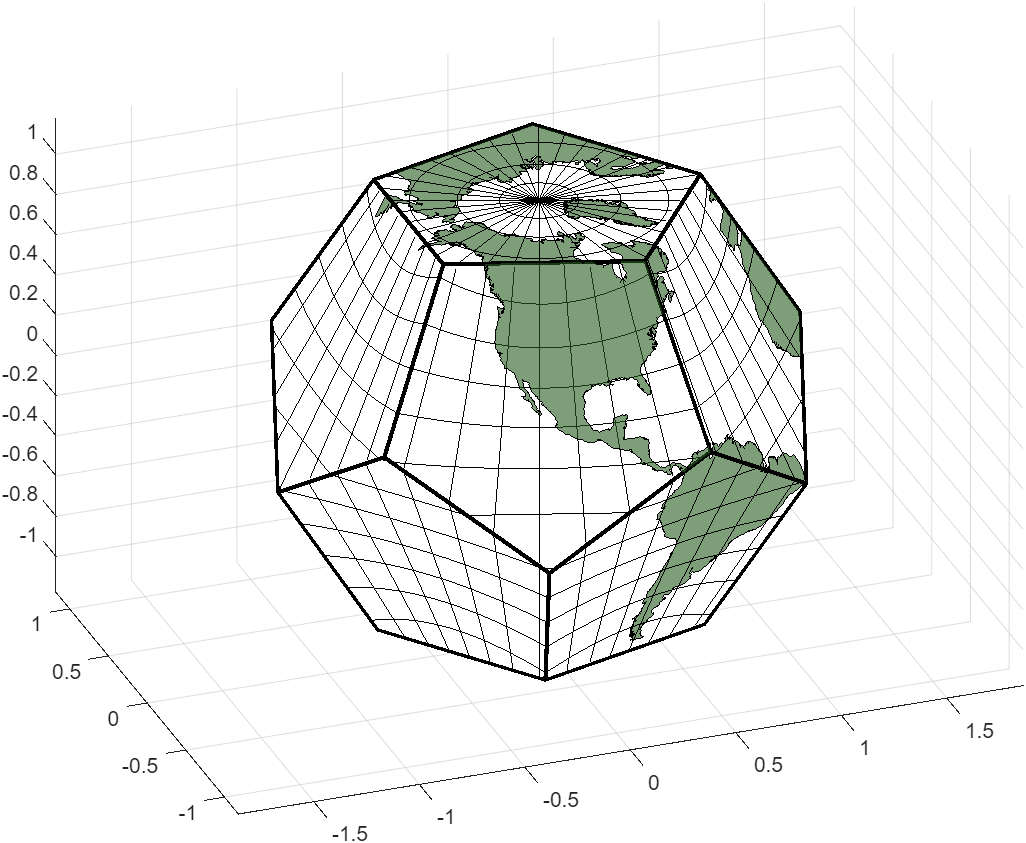
\includegraphics[width=0.8\textwidth]{3D Dodecahedron Globe.png}
    \caption{Finální 3D digitální model glóbu pravidelného dvanáctistěnu}
    \label{fig:3d_globe}
\end{figure}


\subsection{Úprava hlavního skriptu (\texttt{u2.m})}
Hlavní skript \texttt{u2.m} zůstal z matematického a logického hlediska prakticky nezměněn. Definice kroků sítě, výpočet středů jednotlivých stěn i souřadnic vrcholů zůstaly zachovány v původní podobě. Hlavní úprava spočívala v odstranění příkazů \texttt{subplot}, jelikož se model nově nevykresluje do oddělených 2D grafů, ale skládá se dohromady do jednoho společného 3D okna (\texttt{figure}), u kterého je zapnutý 3D pohled a umožněna interakce uživatele.

\subsection{Modifikace funkce \texttt{createGlobeFace.m}}
Tato funkce, původně určená pro vykreslování 2D map, prošla nezbytnou modifikací, aby podporovala 3D vykreslování a eliminovala grafické artefakty gnomonické projekce na okrajích stěn:
\begin{itemize}
    \item \textbf{Ořezání sítě:} Artefakty (čáry směřující do nekonečna) byly odstraněny pomocí funkce \texttt{inpolygon}, která ořízne body poledníků a rovnoběžek přesně na hranici pětiúhelníku. Přesahujícím bodům je přiřazena hodnota \texttt{NaN}, díky čemuž nejsou vykresleny.
    \item \textbf{Ořez a výplň kontinentů:} Funkce \texttt{polyshape} a \texttt{intersect} zajistily přesný ořez kontinentů na hranách stěn. Pro bezchybné vybarvení ploch (včetně složitých tvarů a oddělených ostrovů) byla využita funkce \texttt{triangulation} v kombinaci s \texttt{patch}. Tento postup spolehlivě obchází omezení standardní funkce \texttt{fill3}.
    \item \textbf{3D Vykreslování:} Veškeré 2D příkazy pro kreslení (\texttt{plot}) byly nahrazeny jejich 3D ekvivalenty (\texttt{plot3}).
    \item \textbf{Eliminace Z-fightingu:} Kvůli překrývání vrstev na totožných souřadnicích docházelo k problikávání barev. Řešením bylo mikroskopické oddálení vrstev od středu. Zeměpisná síť byla zvětšena o $0.1\,\%$, pevnina o $0.2\,\%$ a její okraje o $0.3\,\%$. Tím se určil jasný přesah a model se vizuálně vyčistil.
\end{itemize}

\subsection{Nová transformační funkce \texttt{to3D.m}}
Pro zajištění dokonalého lícování stěn byl vytvořen zcela nový pomocný skript \texttt{to3D.m}. Tento skript funguje jako univerzální nástroj pro převod z 2D roviny do 3D prostoru:
\begin{itemize}
    \item Funkce si nejprve vypočítá absolutní 3D souřadnice středu dané stěny na referenční kouli.
    \item Na základě polohy prvních vrcholů pětiúhelníku na kouli a řešení soustavy lineárních rovnic skript dynamicky spočítá správně natočené směrové vektory (lokální osy $X$ a $Y$) pro konkrétní stěnu.
    \item Následně všechny vygenerované 2D souřadnice (zeměpisné sítě i polygonů kontinentů) transformuje pomocí těchto os a umístí je přesně na plášť 3D dvanáctistěnu.
\end{itemize}

\subsection{Využité zdroje}
Při tvorbě prostorového modelu, algoritmizaci a řešení vizualizace složitých polygonů bylo čerpáno z oficiální dokumentace společnosti MathWorks a moderních nástrojů pro asistované programování:
\begin{itemize}
    \item \textbf{Oficiální dokumentace MATLAB (MathWorks)}:
    \begin{itemize}
        \item \textit{2-D and 3-D Plots} -- využití funkcí pro tvorbu prostorových sítí, vizualizaci dat v prostoru a formátování 3D grafů.
        \item \textit{Polygons and Patch Objects} -- implementace geometrických polygonů a triangulace pro spolehlivé vybarvování oříznutých tvarů (včetně eliminace \texttt{NaN} hodnot) pomocí objektů typu \texttt{patch}.
    \end{itemize}
    \item \textbf{Gemini} -- průběžné konzultace a podpora při návrhu algoritmů pro prostorové transformace (převod z 2D roviny na 3D těleso), ladění chyb (debugging) a optimalizaci struktury kódu v prostředí MATLAB (např. automatizované řešení průniků polygonů).
    
\end{itemize}

\clearpage
\newpage

\section{Výsledky}
Pro vlastní tvrobu polyedrických glóbů vybraných platónských těles (krychle a dvanáctistěn) byly spuštěny příslušné skripty \texttt{u2\_hexahedron} pro krychli a \texttt{u2.m} pro dvanáctistěn. Součastí obou skriptů mimo vytvoření jednotlivých stěn přímo v MATLAB byl i export rozloženého tělesa do roviny v měřítku 1 : 150 000 000, aby bylo možné rozložená tělesa vytisknout ve formátu A3. Exporty rozložených těles jsou součástí přílohy. 

Pro správnou velikost bylo nutné zvětšit jednotlivé stěny v prostředí \textbf{SW Inkscape}, ve kterém byly i dané stěny ořezány o segmenty, které spadaly mimo ořezovou plochu. Před slepováním papírového modelu bylo vhodné jednotlivé stěny napojit a vytvořit spojený plášť tělesa. Tento krok by výrazně ulehčil samotné lepení papírového glóbu.

\subsection{Krychle}
V měřítku 1 : 150 000 000 má hrana krychle délku \textbf{8.51 cm}. Pro těleso krychle byly dále spočítány parametry gnómonické projekce, které byly dále porovnány s knihovnout \textit{Proj.4} pomocí konzole \textit{OSGeo4W}. Vypočítané parametry v bodě Q [35.2644°, 45°] jsou zobrazeny v tabulce 2.

\begin{table}[htpb]
\centering
\begin{tabular}{lll}
\hline
parametry šestistěnu & MATLAB & Proj.4 \\ \hline
měřítko v poledníku $m_p$ & 2.999998 & 2.99999847 \\
měřítko v rovnoběžce $m_r$ & 1.732050 & 1.73205037 \\
měřítko ploch $P$ & 5.196148 & 5.19614846 \\
poloosa $a$ Tissotovy indikatrix & 2.999998 & 3.00000 \\
poloosa $b$ Tissotovy indikatrix & 1.732050 & 1.73205 \\
úhel $\omega'$ & 90$^\circ$ 00' 00.00'' & 90.00000° \\
maximální úhlové zkreslení $\Delta\omega$ & 31$^\circ$ 05' 04.28'' & 31.085° \\
meridiánová konvergence $c$ & 0° & 0° \\ \hline
\end{tabular}
\caption{Porovnání parametrů pro šestistěn}
\label{tab:sestisten}
\end{table}


Z tabulky lze vypozorovat zmíněné vztahy zmíněné v teoretické části a také, že naše výpočty jsou správné v porovnání s knihovnou Proj.4.

Pomocí vypočtených parametrů byla dále vytvořena pomocí skriptu \texttt{gnom\_distortions\_hexahedron.m}Tissotova indikatrix v bodě Q (obrázek 5).

\begin{figure}[H]
    \centering
    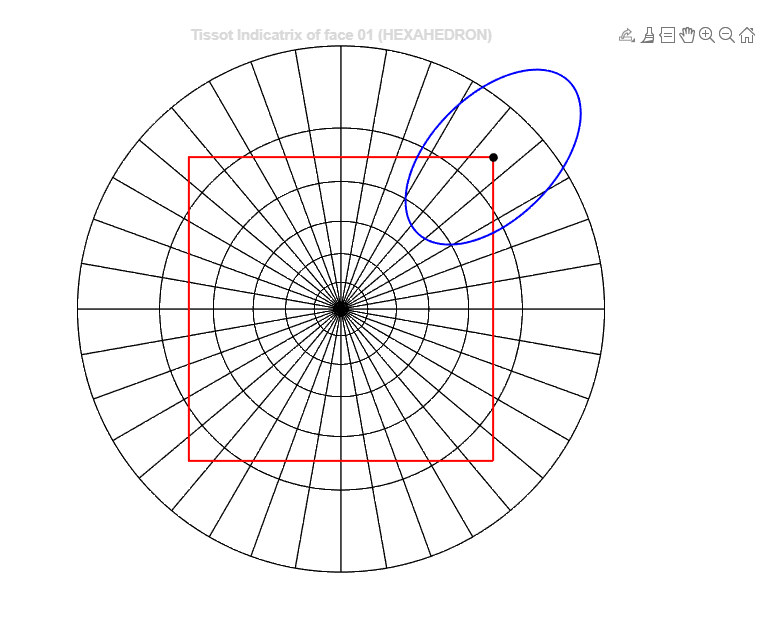
\includegraphics[width=0.8\textwidth]{hexa_tissot.png}
    \caption{Tissotova indikatrix pro těleso krychle}
    \label{fig:hex_tissot}
\end{figure}

\subsection{Dvanáctistěn}
Dvanáctistěn má v měřítku 1 : 150 000 000 délku své hrany \textbf{3.82 cm}. Obdobně jako pro krychli byly i pro dvanáctistěn vypočítány vlastnosti gnómonické projekce v bodě Q [52.6226°, 0°] pomocí skriptu \texttt{gnom\_distortions\_dodecahedron.m}. Námi vypočtené parametry byly opět srovnány s knihovnou \textit{Proj.4} a byly zobrazeny v tabulce 4 níže.


\begin{table}[htpb]
\centering
\begin{tabular}{lll}
\hline
dvanáctistěn & MATLAB & Proj.4 \\ \hline
měřítko v poledníku mp & 1.583593 & 1.58359348 \\
měřítko v rovnoběžce mr & 1.258409 & 1.25840911 \\
měřítko ploch P & 1.992808 & 1.99280846 \\
poloosa a Tissotovy indikatrix & 1.583593 & 1.58359 \\
poloosa b Tissotovy indikatrix & 1.258409 & 1.25841 \\
omega' & 90$^\circ$ 00' 00.00'' & 90.00000$^\circ$ \\
maximální úhlové zkreslení & 13$^\circ$ 08' 25.60'' & 13.140$^\circ$ \\
meridiánová konvergence & 45$^\circ$ & 45$^\circ$ \\ \hline
\end{tabular}
\caption{Porovnání hodnot pro dvanáctistěn}
\label{tab:dvanactisten}
\end{table}

Opět lze z tabulky pozorovat, že se parametry neliší a tudíž naše výpočty byly správné.

Díky těmto parametrům byla opět vytvořena Tissotova indikatrix v bodě Q (obrázek 6).

\begin{figure}[H]
    \centering
    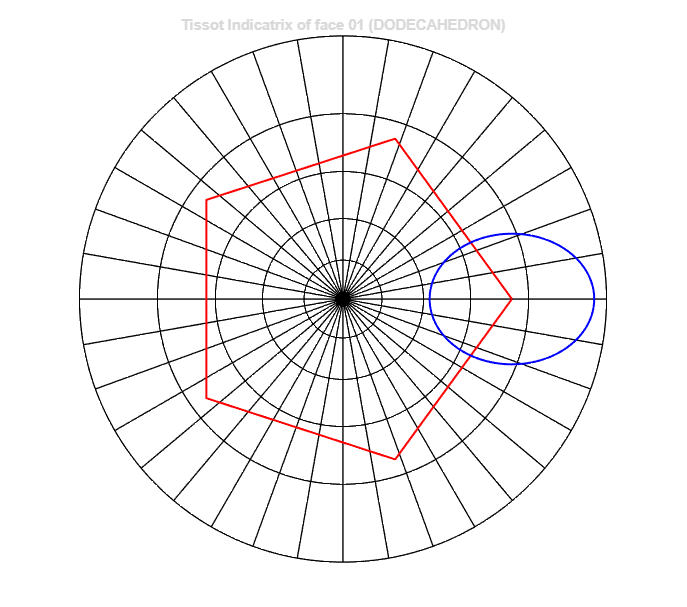
\includegraphics[width=0.8\textwidth]{dodeca_tissot.png}
    \caption{Tissotova indikatrix pro těleso dvanáctistěnu}
    \label{fig:dodeca_tissot}
\end{figure}

Při porovnání tabulek 3 a 4 či vizuálním porovnání obrázků 5 a 6, tedy porovnání zkreslení lze pozorovat, že se ve zvolených bodech elipsy dosti liší. V krajním bodě krychle je elipsa výrazně protáhlejší než v případě dvanáctistěnu.

\section{Závěr}
Úkolem této úlohy bylo vytvoření polyedrických glóbů šesti- a dvanáctistěnu. Bylo nutné se seznámit s teoretickým základem gnómografické projekce, výpočty a generovnání geografické sítě a kontinetnů. Dále bylo potřeba vlastní výpočty parametrů zvolené projekce zkontrolovat s knihovnou  \textit{Proj.4} pro ověření správnosti výsledků. Všechny skripty byly realizovány v SW MATLAB, které jsou v přílohách. Pomocí vypočítaných parametrů byly ve vybraných bodech vykresleny indikátory zkreslení - Tissotovy indikatrix.

Vzniklé glóby splňují zadání i rozměry ve zvoleném měřítku 1 : 150 000 000. Výranou nevýhodou při samotném lepení glóbu byl fakt, že stěny nebyly k sobě nalícovýny již při exportu. Tento problém způsobil náročnější skládání papírových glóbů.

Bonusově byl globus dvanáctistěnu převeden do 3D prostředí jednak v MATLAB tak i následně vyexportován i pro prohlížení ve webovém prostředí (např. 3DViewer.net).

Přestože skripty fungují spolehlivě, bylo by dále vhodné rozšířit možnosti volby výpočtu pro další jednotlivá zobrazení či výběr dalších platónských těles. Vhodné by bylo i přidání možnost volby bodu Q uživatelem pro výpočty parametrů zobrazení.

\section{Přílohy}

\textbf{MATLAB skripty}

\begin{itemize}
    \item \texttt{uvTosd.m} - převádí zeměpisné souřadnice na kartografické podle kartografického pólu
    
    \item \texttt{gnom.m} - realizuje gnomonickou projekci v obecné poloze
    
    \item \texttt{continent.m} - načítá a promítá lomové body kontinentů z jednotlivých textových souborů
    
    \item \texttt{createGlobeFace.m} - vykresluje jednotlivé plošky glóbu se sítí, kontinenty a ořezovými hranami
    
    \item \texttt{gnom\_distortions\_hexahedron.m} - vypočítává parametry projekce včetně Tissotovy indikatrix pro krychli
    
    \item \texttt{gnom\_distortions\_dodecahedron.m} - vypočítává parametry projekce včetně Tissotovy indikatrix pro dvanáctistěn
    
    \item \texttt{boundary.m} - definuje a vykresluje ořezové linie
    
    
    \item \texttt{graticule.m} - generuje síť poledníků a rovnoběžek v zadaném rozsahu a rozlišení
    
    \item \texttt{u2.m} - hlavní skript pro sestavení všech 12 plošek dvanáctistěnu
    
    \item \texttt{u2\_hexahedron.m} - hlavní skript pro sestavení všech 12 plošek krychle

    \item \texttt{u2\_proj4\_bonus.m} - slouží k validaci vlastního výpočtu zkreslení gnómonické projekce a generuje příkaz pro ověření v knihovně \textit{Proj.4}
    
\end{itemize}

\textbf{Textové soubory kontinentů}

\begin{itemize}
    \item \texttt{afr.txt}
    \item \texttt{afr\_mad.txt}
    \item \texttt{amer.txt}
    \item \texttt{antar.txt}
    \item \texttt{austr.txt}
    \item \texttt{eur.txt}
    \item \texttt{greenl.txt}
    \item \texttt{newzel1.txt}
    \item \texttt{newzel2.txt}
    \item \texttt{tasm.txt}
\end{itemize}

\textbf{Exporty}

\begin{itemize}
    \item \texttt{3D\_dodecahedron.fig} - 3D model dvanáctistěnu v prostředí MATLAB
    \item \texttt{dodecaedr\_faces.svg} - export neupravených stěn dvanáctistěnu z MATLAB ve formátu .svg
    \item \texttt{dodecaedr\_faces\_final.svg} - upravené stěny dvanáctistěnu z Inkscape ve formátu .svg (případeně .pdf)
    \item \texttt{hexahedron\_faces.svg} - export neupravených stěn krychle z MATLAB ve formátu .svg
    \item \texttt{hexahedron\_faces\_final.svg} - upravené stěny krychle z Inkscape ve formátu .svg (případeně .pdf)
    \item \texttt{tissot\_dodecahedron} - stěna dvanáctistěnu s Tissotovou indikatrix v bodě Q
    \item \texttt{tissot\_hexahedron} - stěna krychle s Tissotovou indikatrix v bodě Q
\end{itemize}

\printbibliography[title=Zdroje]
\end{document}